

\begin{frame}[ctb!]
  \frametitle{Heat Limits In Geology}
  % table?
  Important heat limits in materials of the repository restrict loading designs 
  and capacity.
  %        File: heat_tab.tex
%     Created: Thu Aug 04 11:00 AM 2011 C
% Last Change: Thu Aug 04 11:00 AM 2011 C
%
\begin{table}[h!]
  \centering
  \footnotesize{
  \begin{tabular}{|l|r|r|r|r|}
    \multicolumn{5}{c}{\textbf{Thermal Behavior of Various Concepts}}\\
    \hline
    Feature & Clay & Granite & Salt & Deep Borehole \\ 
    \hline
    Buffer Limit $[^{\circ}C]$ & 100 (Fo-Ca) & 100 (Fo-Ca) & 180 & 100 (Fo-Ca) \\ 
    Host Limit $[^{\circ}C]$   & 100 (alteration)  & 200 (cracking) & 180 (brines) & none \\ 
    Conductivity $[\frac{W}{m{\cdot}K}]$ & $1-2$ & $2-4$ & $\sim4$  & $2-4$ \\ 
    Coalesence & yes & no & yes & no \\ 
    \hline
  \end{tabular}
  }
  \label{tab:heat_tab}
\end{table}

\end{frame}

% heat based capacity 
\begin{frame}[ctb!]
  \frametitle{Impact of Repository Designs}
  % lines, points, infinite lines, footprints.
   \input{../report/litrev/footprint_tab.tex}
   \begin{figure}[h!]
     \begin{center}
       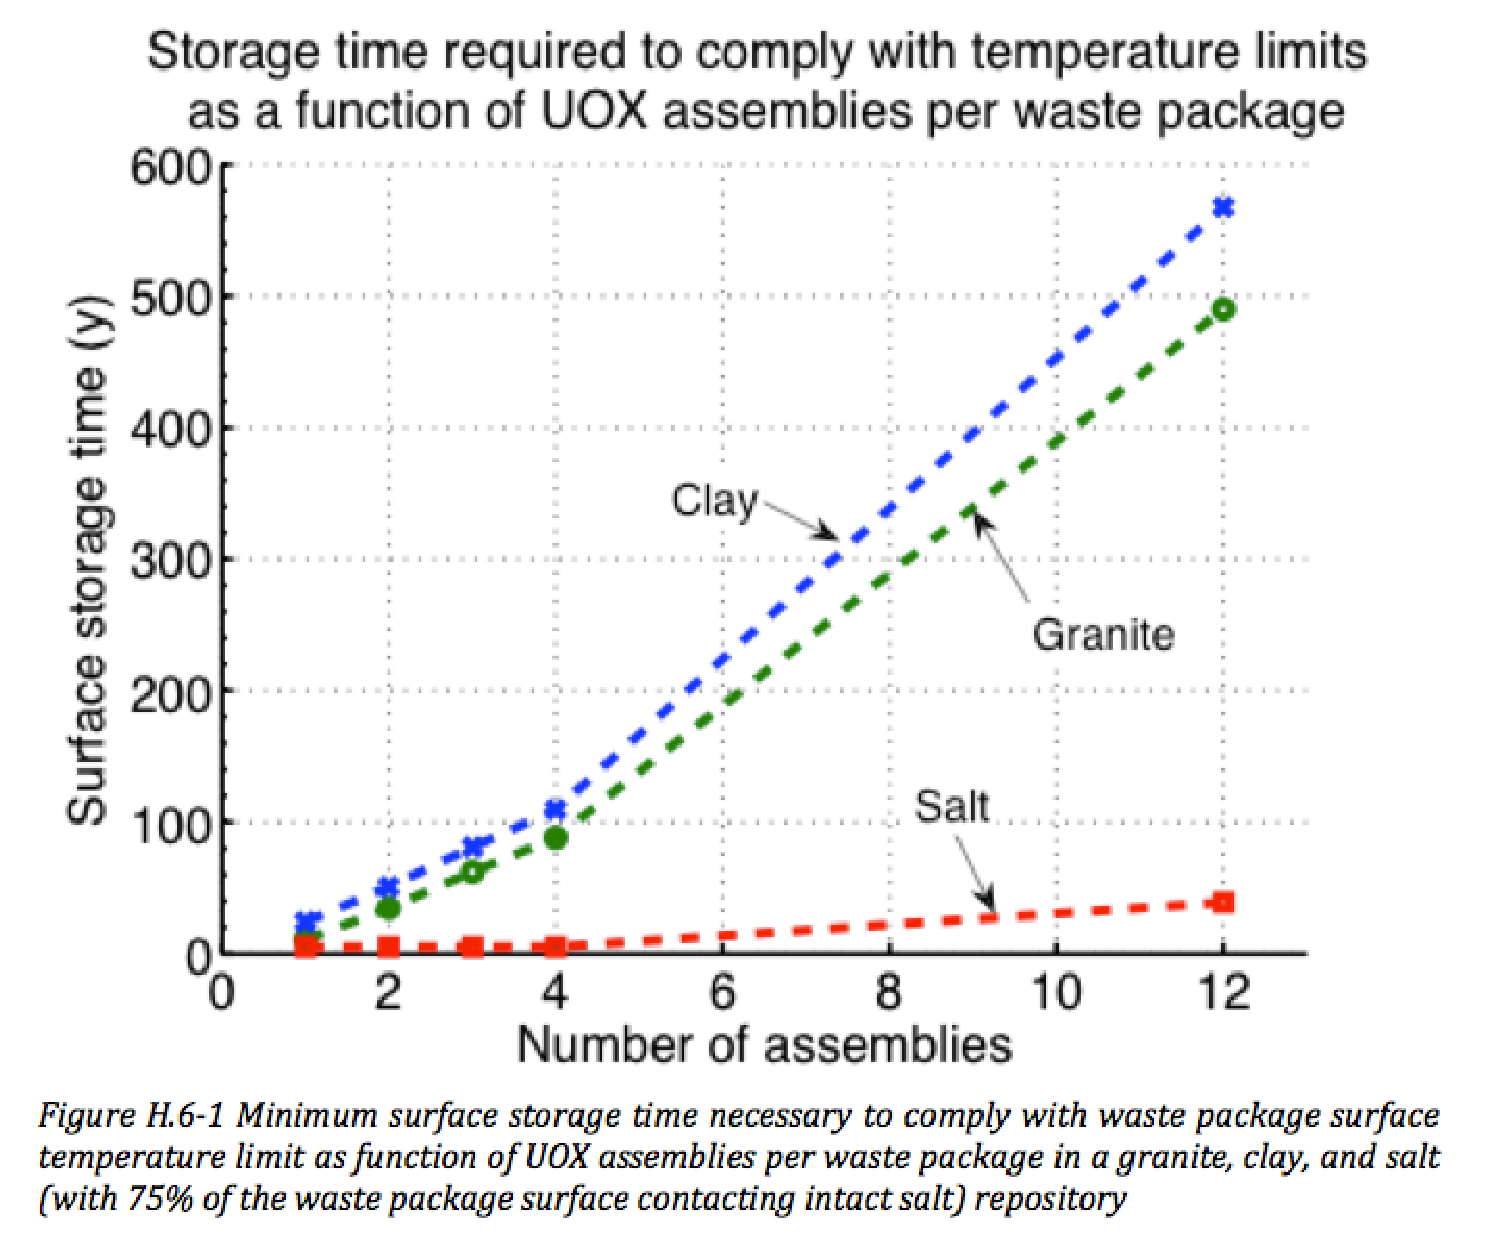
\includegraphics[height=.5\textheight]{llnlGeos.eps}
     \end{center}
     \caption{LLNL has found that the higher heat limit, alcove geometry, and 
     high conductivity in salt allows for earlier loading times.}
     \label{fig:llnlGeos}
   \end{figure}
\end{frame}

% heat based capacity 
\begin{frame}[ctb!]
  \frametitle{Heat Based Capacity}
  % lines, points, infinite lines, footprints.
  \begin{minipage}{0.49\textwidth}
    \begin{figure}[h!]
        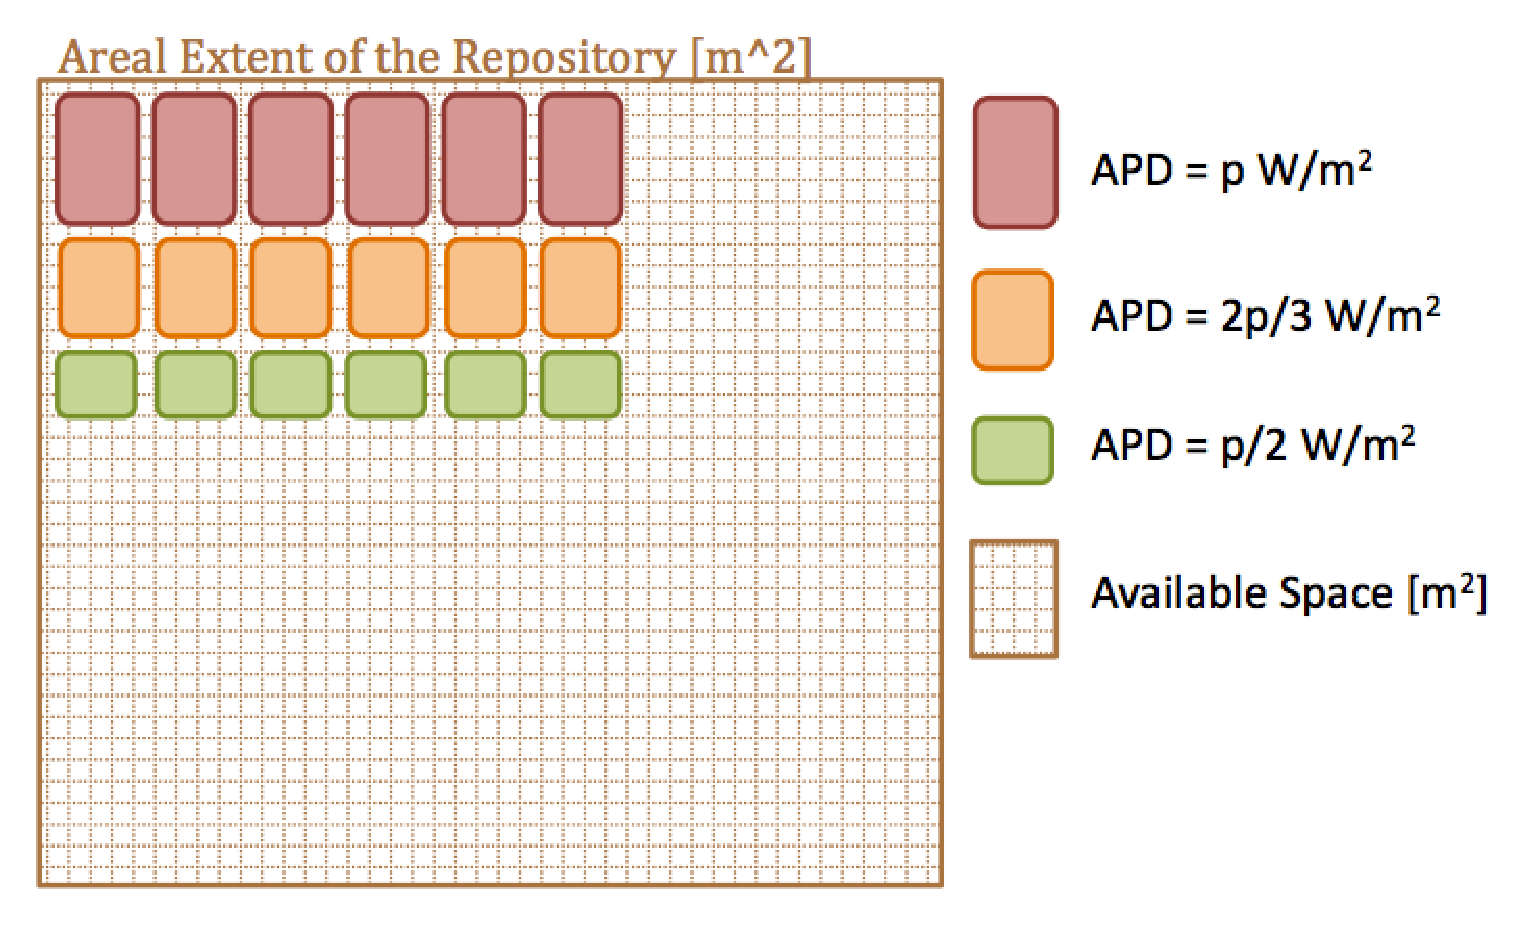
\includegraphics[width=0.9\textwidth]{APD.eps}
      \caption{Areal Power Density (APD) can be used to determine appropriate 
      repository loading for arbitrary waste streams. }
      \label{fig:apd}
  \end{figure}
  \end{minipage}
  \hspace{0.01cm}
  \begin{minipage}{0.49\textwidth}
    Loading is subject to the constraints,
    \footnotesize{
    \begin{align}
      P_{tot} &\le P_{max} \\
      APD_i &\le APD_{max}
      \intertext{where}
      P_{max} &= A\cdot APD_{max}\\ 
      P_{tot} &= \sum_{i=0}^{N}n_i P_i\\ 
      P_i &= \mbox{power of package i}\nonumber\\
      n_i &= \mbox{ith package}\nonumber\\
      N &= \mbox{number of packages}\nonumber\\
      APD_{max} &= \mbox{max areal power density}\nonumber
    \end{align}
    }
  \end{minipage}
\end{frame}

\begin{frame}[ctb!]
  \frametitle{Detailed Techniques}
  % 2d,3d,finite diffs, etc.
  %        File: heat_tab.tex
%     Created: Thu Aug 04 11:00 AM 2011 C
% Last Change: Thu Aug 04 11:00 AM 2011 C
%
\begin{table}[h!]
  \centering
  \footnotesize{
  \begin{tabular}{|l|r|r|r|r|}
    \multicolumn{5}{c}{\textbf{Thermal Behavior of Various Concepts}}\\
    \hline
    Feature & Clay & Granite & Salt & Deep Borehole \\ 
    \hline
    Buffer Limit $[^{\circ}C]$ & 100 (Fo-Ca) & 100 (Fo-Ca) & 180 & 100 (Fo-Ca) \\ 
    Host Limit $[^{\circ}C]$   & 100 (alteration)  & 200 (cracking) & 180 (brines) & none \\ 
    Conductivity $[\frac{W}{m{\cdot}K}]$ & $1-2$ & $2-4$ & $\sim4$  & $2-4$ \\ 
    Coalesence & yes & no & yes & no \\ 
    \hline
  \end{tabular}
  }
  \label{tab:heat_tab}
\end{table}

  Similar heat transport models can be used for all geologies, but are 
  differentiated by material parameters $(c_p, K, \rho)$ and different 
  thermal constraints.
\end{frame}


% SINDA 

\begin{frame}
  \frametitle{ANL model}
  A model created by the UFD team at Argonne national lab using the 
  SINDA{\textbackslash}G heat transport framework employs a lumped parameter 
  model and an optimization loop to arrive at a minimal drift spacing for a 
  given waste stream in agreement with user input thermal limits. 
  \begin{figure}[h!]
    \begin{center}
      \includegraphics[height=.5\textheight]{../report/litrev/sindageom.eps}
    \end{center}
    \caption{Two adjustable geometric dimensions of the ANL model.} 
    \label{fig:sindageom}
  \end{figure}
\end{frame}


\begin{frame}[ctb!]
  \frametitle{Lumped Parameter Technique}
  % resistor diagram
  \begin{figure}[h!]
    \begin{center}
      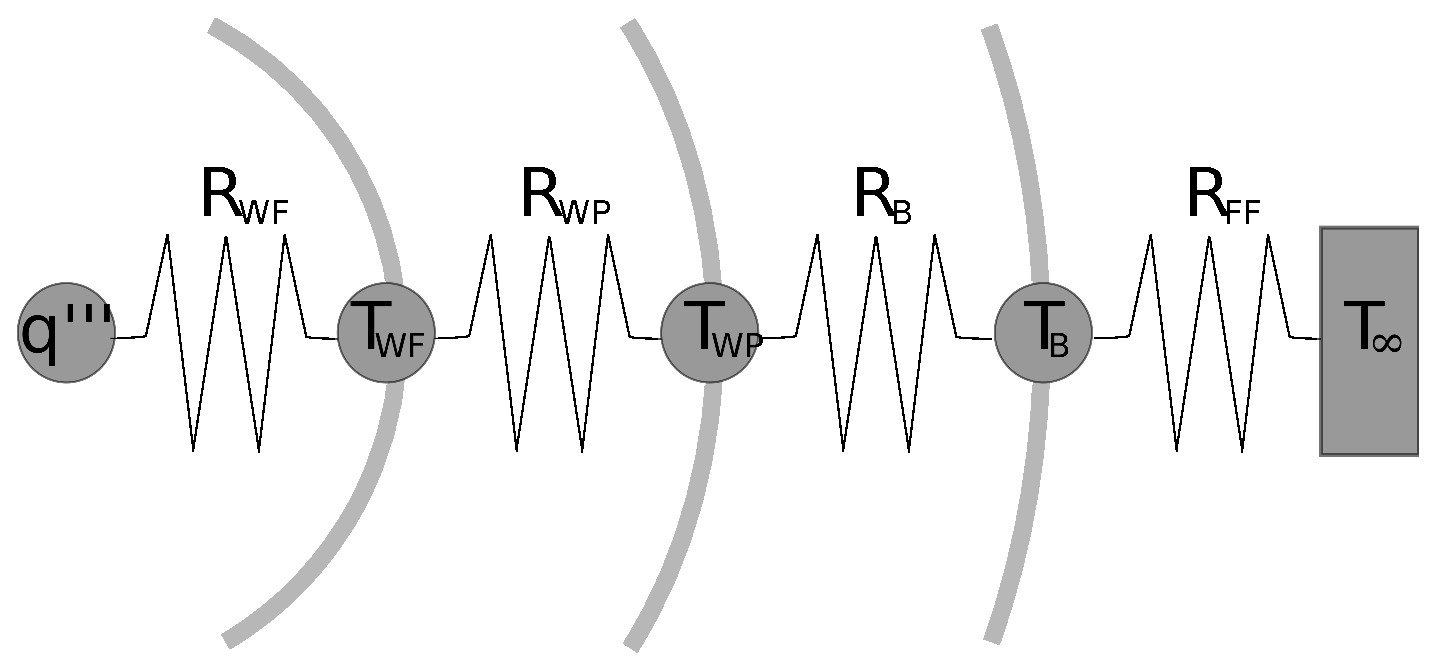
\includegraphics[width=0.9\textwidth]{lumpedParam.eps}
    \end{center}
    \caption{The lumped parameter analogy used for heat transfer can be applied 
    as a one dimensional approximation to the disposal system concept. }
    \label{fig:lumpedParam}
  \end{figure}
\end{frame}


% LLNL

\begin{frame}
  \frametitle{LLNL Model : Geometry}
  \begin{minipage}{0.3\textwidth}
    \begin{figure}[h!]
      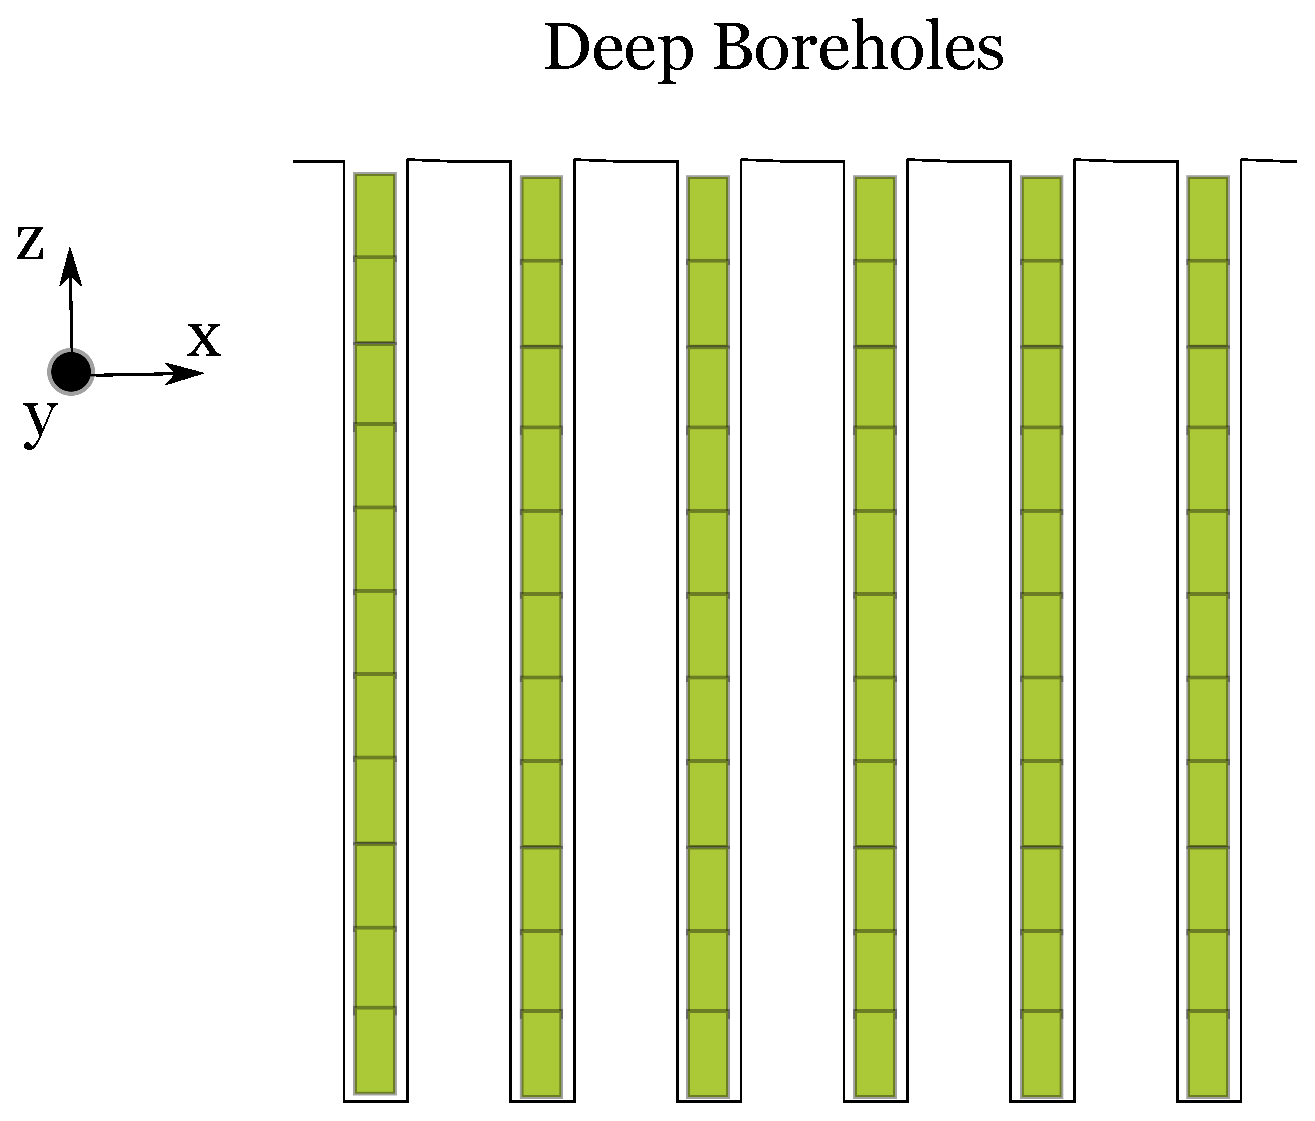
\includegraphics[width=\textwidth]{boreholes.eps}
    \end{figure}
    \begin{figure}[h!]
      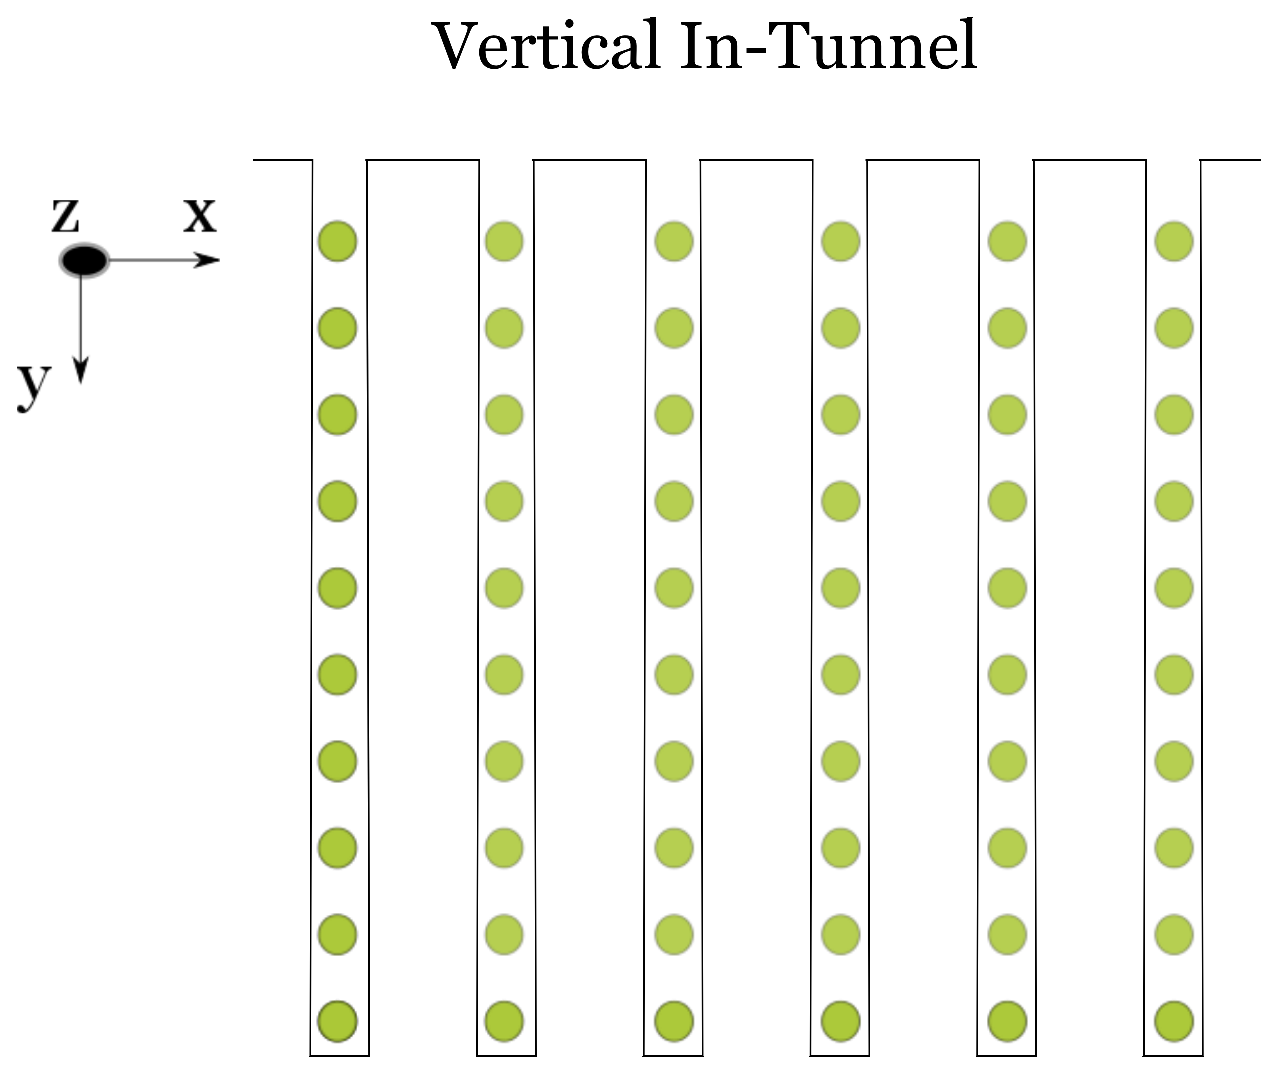
\includegraphics[width=\textwidth]{vertical.eps}
    \end{figure}
  \end{minipage}
  \hspace{0.01cm}
  \begin{minipage}{0.3\textwidth}
    \begin{figure}[h!]
      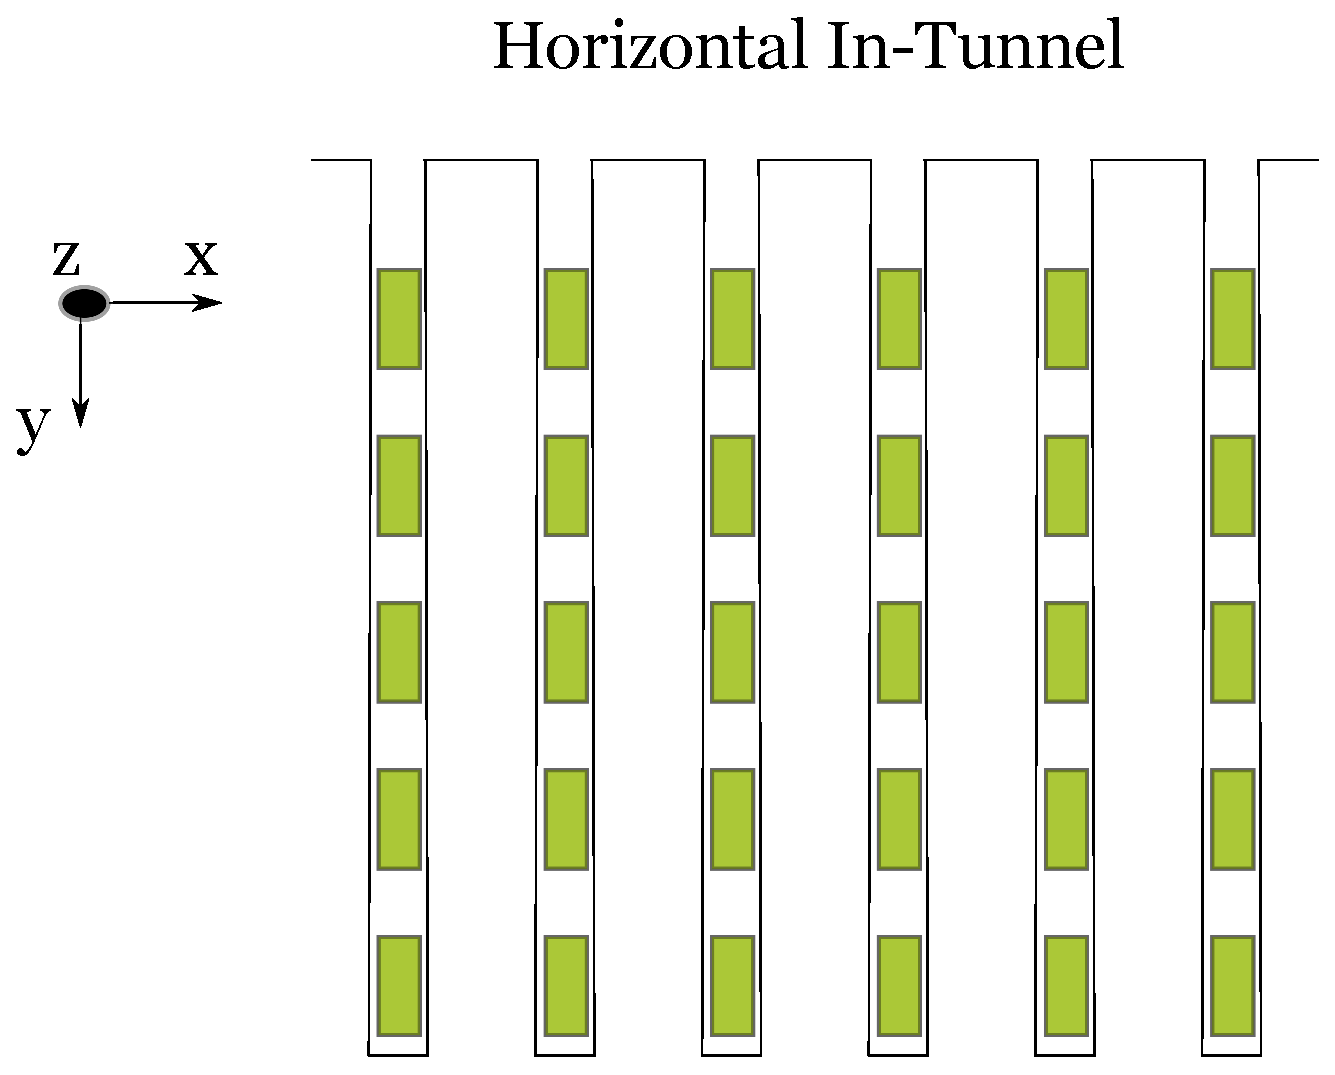
\includegraphics[width=\textwidth]{horizontal.eps}
    \end{figure}
    \begin{figure}[h!]
      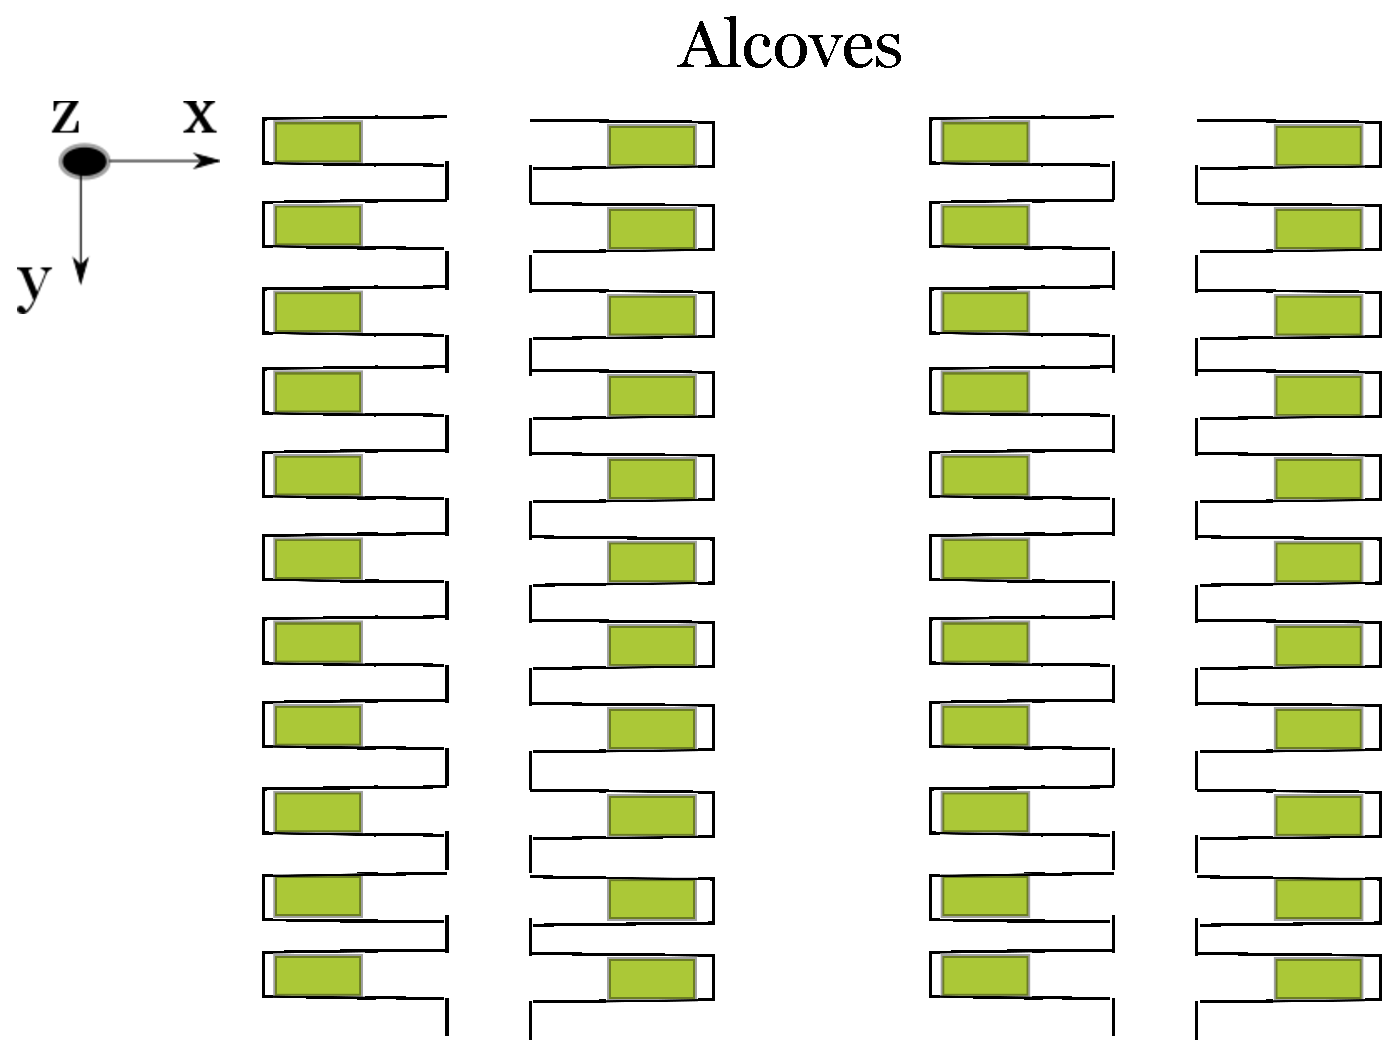
\includegraphics[width=\textwidth]{alcoves.eps}
    \end{figure}
  \end{minipage}
  \hspace{0.01cm}\large{$=$}\hspace{0.01cm}
  \begin{minipage}{0.3\textwidth}
    \begin{figure}[b]
      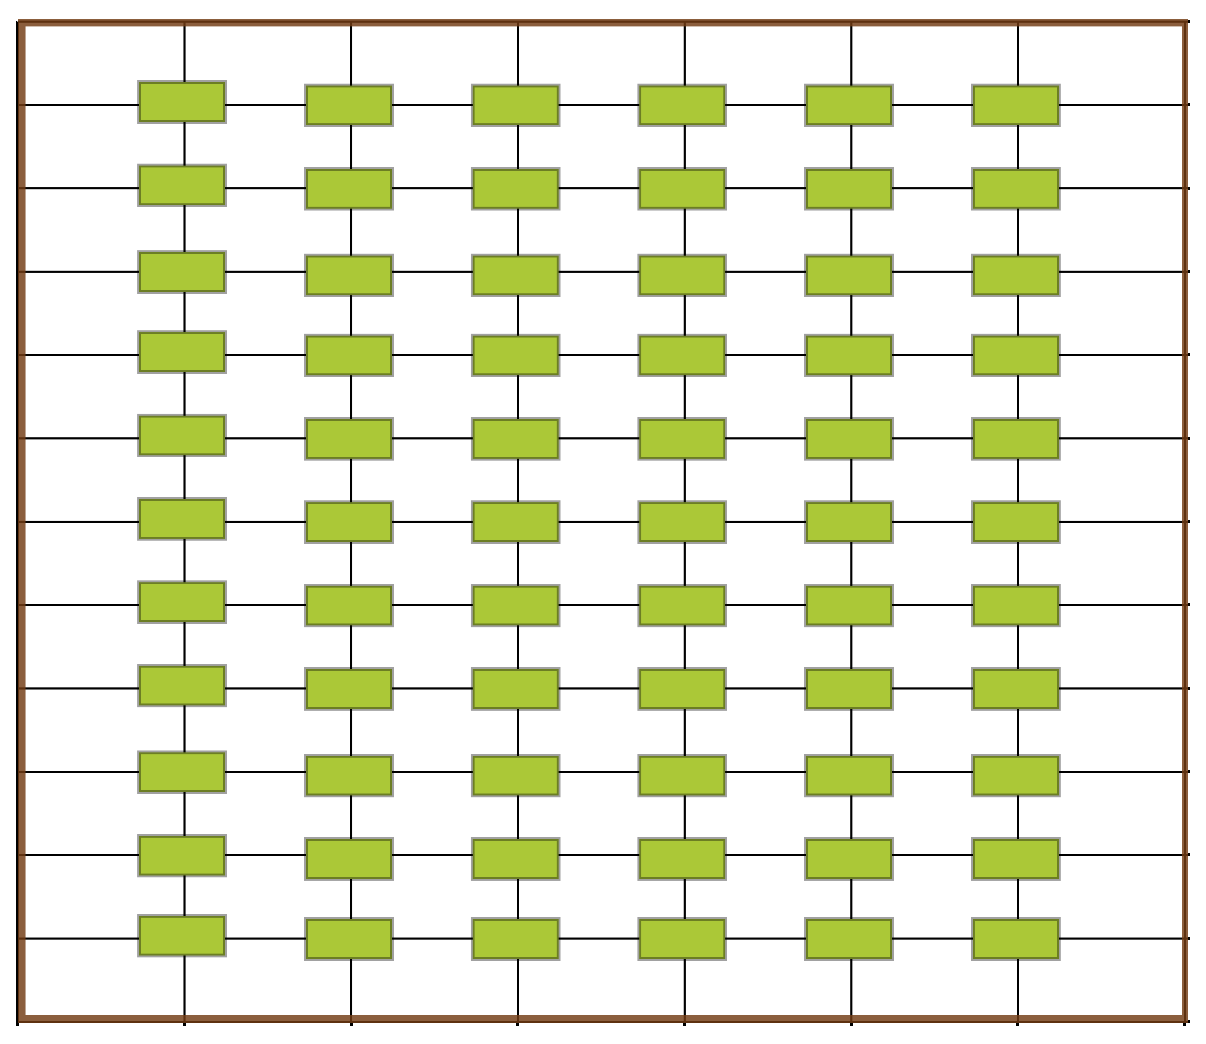
\includegraphics[width=\textwidth]{fullGrid.eps}
    \end{figure}
  \end{minipage}
\end{frame}

\begin{frame}
  \frametitle{LLNL Model : Geometry}
  \begin{figure}[h!]
    \begin{center}
      \includegraphics[width=0.7\textwidth]{llnlConcept.eps}
    \end{center}
    \caption{Vertical, horizontal, alcove, and borehole emplacement layouts can 
    be represented by a line of point sources and adjacent line sources 
    \cite{sutton_investigations_2011}.}
    \label{fig:llnl}
  \end{figure}
\end{frame}

\begin{frame}
  \frametitle{LLNL Model : Solution Strategy}
  \footnotesize{
    LLNL's model is a MathCAD solution of the transient homogeneous 
    conduction equation,
    
    \begin{align}
      \nabla^2T  = \frac{1}{\alpha}\frac{\partial T}{\partial t},
      \label{condGl}
    \end{align}
    
    in which superimposed point and line source solutions approximate the repository 
    layout.
    The solution of this equation at the 
    boundary of the EBS and the waste package is then treated as a boundary condition 
    for the heterogeneous steady state equation, 
    
    \begin{align}
      \dot{q} &= U A_{out} \left( T_{in} - T_{out} \right)
      \label{condGeneral}
      \intertext{where}
      U&=\frac{1}{\sum_{i}R_i}
      \intertext{which, for the detailed EBS becomes}
      U&=\frac{1}{R_{WF}+R_{WP}+R_{buffer}+\cdots}
    \end{align}
    
    which calculates a resulting temperature gradient through the geometry at each 
    point in time for each layer surface, assuming an infinite line source 
    \cite{hardin_generic_2011}\cite{sutton_investigations_2011}. 
    }
\end{frame}



